\documentclass[12pt, twoside]{article}
\usepackage[letterpaper, margin=1in, headsep=0.5in]{geometry}
\usepackage[english]{babel}
\usepackage[utf8]{inputenc}
\usepackage{amsmath}
\usepackage{amsfonts}
\usepackage{amssymb}
\usepackage{tikz}
\usepackage{yhmath}
\usetikzlibrary{quotes, angles}
\usepackage{graphicx}
\usepackage{enumitem}
\usepackage{multicol}

\newif\ifmeta
\metatrue %print standards and topics tags

\title{Regents Geometry}
\author{Chris Huson}
\date{March 2022}

\usepackage{fancyhdr}
\pagestyle{fancy}
\fancyhf{}
\renewcommand{\headrulewidth}{0pt} % disable the underline of the header
\raggedbottom

\fancyhead[LE]{\thepage}
\fancyhead[RO]{\thepage \\ Name: \hspace{4cm} \,\\}
\fancyhead[LO]{BECA / Dr. Huson / Geometry\\* Unit 10: Trigonometry\\* 7 April 2022}

\begin{document}
\subsubsection*{10.4 Do Now Quiz: Trigonometric functions \hfill HSG.SRT.C.8}
\begin{enumerate}
\item Right triangle $\triangle ABC$ is shown with side lengths marked. Identify the sides. \vspace{0.5cm}
\begin{multicols}{2}
  \begin{enumerate} [itemsep=1cm]
    \item Which length is the hypotenuse?
    \item Which length is \emph{opposite} angle $A$?
    \item Which length is \emph{adjacent} to angle $A$?
  \end{enumerate}
\begin{flushright}
        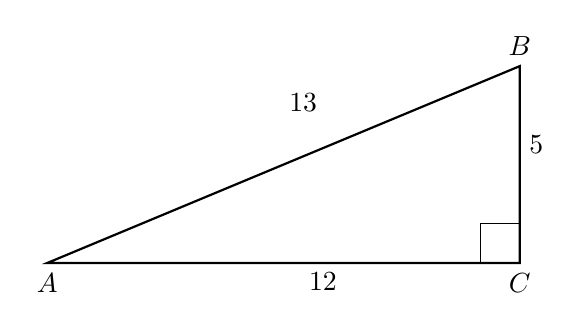
\begin{tikzpicture}[scale=1]
        \draw [thick]
        (0,0)node[below]{$A$}--
        (6,0)node[below]{$C$}--
        (6,2.5)node[above]{$B$}--cycle;
        \draw (6,0)++(-0.5,0)--++(0,0.5)--+(0.5,0);
        \node at (3.5,0)[below]{$12$};
        \node at (6,1.5)[right]{$5$};
        \node at (3.25,1.8)[above]{$13$};
      \end{tikzpicture}
\end{flushright}
\end{multicols}  \vspace{1cm}

\item $\triangle ABC$ is shown with $m\angle C=90^\circ$. The lengths of the triangle's sides are $a$, $b$, and $c$. Express each trigonometric ratio as a fraction of two lengths. \vspace{1cm}
\begin{multicols}{2}
    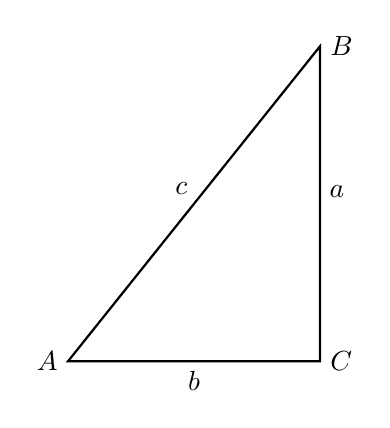
\begin{tikzpicture}[scale=0.8]
      \draw [thick]
      (0,0)node[left]{$A$}--
      (4,0)node[right]{$C$}--
      (4,5)node[right]{$B$}--cycle;
      \node at (2,0)[below]{$b$};
      \node at (4,2.7)[right]{$a$};
      \node at (1.8,2.5)[above]{$c$};
    \end{tikzpicture}
      \begin{enumerate}
        \item $\tan A =$ \vspace{0.75cm}
        \item $\sin A =$ \vspace{0.75cm}
        \item $\cos A =$ \vspace{0.75cm}
    \end{enumerate}
\end{multicols} \vspace{0.5cm}

\item Express the result to \emph{the nearest thousandth}.
\begin{multicols}{2}
  \begin{enumerate}
    \item $\tan 81^\circ =$
    \item $\sin 16^\circ =$
  \end{enumerate}
\end{multicols} \vspace{1cm}

\item Express the result to \emph{the nearest whole degree}.
\begin{multicols}{2}
  \begin{enumerate}
    \item $\sin^{-1} 0.675 =$
    \item $\tan^{-1} 1.15 =$
  \end{enumerate}
\end{multicols}

\newpage
\subsubsection*{Early finishers / test corrections \hfill HSA.REI.B.3}
\item Are the lines parallel, perpendicular, or neither? Justify your answer. \\(you must use the values of the slopes in your justification)
  \begin{multicols}{2}
    $y = -\frac{5}{3}x+5$ \\
    $y = \frac{3}{5}x-4$
  \end{multicols} \vspace{3cm}

\item Given $P(1,7)$ and $Q(5,5)$, find the length of $\overline{PQ}$, expressed as a simplified radical.\\[0.25cm]
Use: $l=\sqrt{(x_2-x_1)^2+(y_2-y_1)^2}$
    \vspace{4cm}

\item A translation $T_{x,y}$ maps $A(6,2) \rightarrow A'(3,7)$. 
\begin{enumerate}
  \item Write down the translation. \vspace{1cm}
  \item Apply the same translation to $B(5, 1)$.
\end{enumerate} \vspace{2cm}

\item $A(2,3)$ is one endpoint of $\overline{AB}$. The segment's midpoint is $M(5,7)$. Find the other endpoint $B$. (hint: find the translation that maps $A \rightarrow M$, then apply it to map $M \rightarrow B$.)

\end{enumerate}
\end{document}
  